\title{バージョン管理システムチュートリアル}

\begin{document}

\lstset{language={sh},basicstyle=\ttfamily\footnotesize,showspaces=false,rulecolor=\color[cmyk]{0, 0.29,0.84,0}}

\begin{frame}
  \titlepage
  \noindent {\footnotesize ソースコード: \url{https://github.com/cmsi/vcs-tutorial}} \\
  \noindent {\footnotesize 資料作成: \url{https://github.com/cmsi/vcs-tutorial/graphs/contributors}}
\end{frame}

\section*{Outline}
\begin{frame}
  \tableofcontents
\end{frame}

\section{準備作業}

\begin{frame}
  \frametitle{ネットワーク設定・MateriApps LIVE! 設定}
  \begin{itemize}
    \setlength{\itemsep}{1em}
  \item LAN接続 (無線 or 有線)
  \item GitHub アカウント登録 (まだアカウントを持っていない人のみ)
    \begin{itemize}
    \item \url{https://github.com} にアクセス
    \item ``Sign up for GitHub''をクリック, 必要事項を記入した後, ``Create an account''
    \item (オプション) SSH公開鍵の登録 (``Account settings'' $\Rightarrow$ ``SSH Keys'')
    \end{itemize} 
  \item MateriApps LIVE! の設定
    \begin{itemize}
      \item \href{http://www.slideshare.net/cms_initiative/materiapps-live-52477264}{「MateriApps LIVE! の設定」}に従い、VirtualBox、MateriApps LIVE! をインストール・設定
    \end{itemize}
  \end{itemize}
\end{frame}

\begin{frame}[t,fragile]
  \frametitle{WindowsやMac上で直接gitを使いたい場合}
  \begin{itemize}
    %\setlength{\itemsep}{1em}
  \item Windows \& Mac OS X
    \begin{itemize}
      \item \url{http://git-scm.com/downloads}からインストーラーをダウンロード
      \item \url{https://www.sourcetreeapp.com/}からSourceTreeをインストール
      \item Mac の場合は MacPorts からインストールすることも可
\begin{lstlisting}
$ sudo port install git
\end{lstlisting}
    \end{itemize}
  \item Linux
    \begin{itemize}
      \item Redhat系
\begin{lstlisting}
$ sudo yum install git
\end{lstlisting}
      \item Debian系
\begin{lstlisting}
$ sudo apt-get install git
\end{lstlisting}
    \end{itemize}
  \end{itemize}
\end{frame}

\section{バージョン管理システムとは?}

\begin{frame}[t,fragile]{バージョン管理システムの必要性}
  \begin{itemize}
    \setlength{\itemsep}{1em}
  \item 広く行われている「ファイル管理」
    \begin{itemize}
    \item ファイル名・ディレクトリ名による管理

      (日付、人名、バージョン番号など)
    \item 手書きのログファイルによる記録
    \end{itemize}
  \item 問題点
    \begin{itemize}
    \item 記録を付け忘れる、記録を間違う、不完全な記録
    \item 人により命名規則がばらばら
    \item コンピュータ間でコピーを繰り返すと、どれを修正したか、どれが新しいか分からなくなる
    \item 同じバージョンを元に、別の人が独立に修正を行ってしまう

      (バージョンの分岐)
    \end{itemize}
  \end{itemize}
\end{frame}

\begin{frame}
  \frametitle{ありがちなパターン}
  \begin{center}
    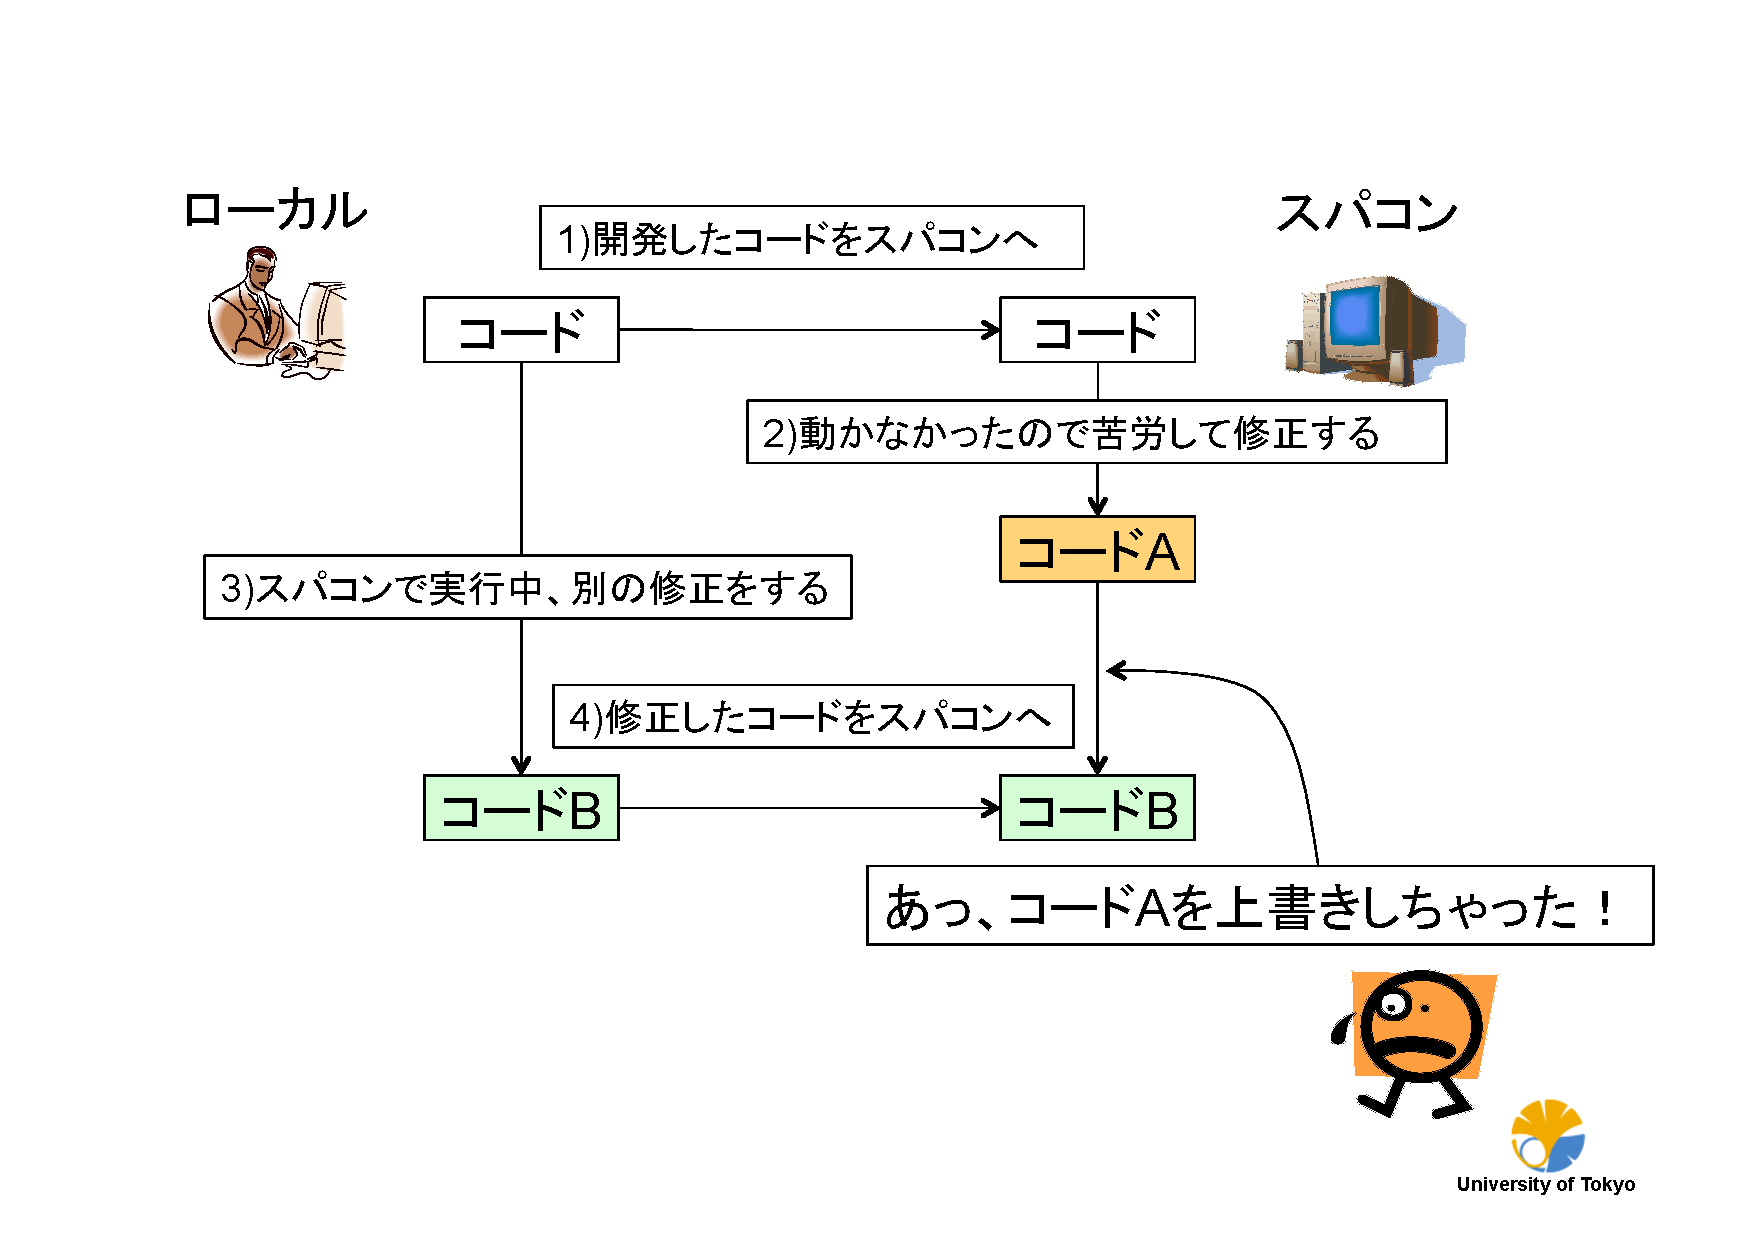
\includegraphics[height=0.88\textheight]{pattern-1.pdf}
  \end{center}
\end{frame}

\begin{frame}[t,fragile]{バージョン管理システム(Version Control System)とは?}
  \begin{itemize}
    \setlength{\itemsep}{1em}
  \item ファイルの履歴をデータベース(リポジトリ)で一括管理するシステム
    \begin{itemize}
    \item 全ての修正履歴(差分)を保存
    \item 更新毎に一意なバージョン番号(リビジョン)を付与
    \item 任意のバージョン間の比較が可能
    \item もともとはプログラムのソースコードのためのシステム
    \item それ以外のファイル(例えば TeX ファイル)管理にも使える
    \end{itemize}
  \item チーム・分散環境での作業をサポート
    \begin{itemize}
    \item ネットワーク経由でファイルを check out/check in
    \item 複数箇所から同時に更新した場合に衝突を回避するしくみ
    \item ブランチ・マージ・タグの管理
    \item 一人で使っても複数人で使っても超便利
    \item 超優秀な(かつ超まじめな)秘書のようなもの (しかもタダ)
    \end{itemize}
  \end{itemize}
\end{frame}

\begin{frame}[t,fragile]{バージョン・ブランチ・マージ}
  \begin{center}\resizebox{!}{0.8\textheight}{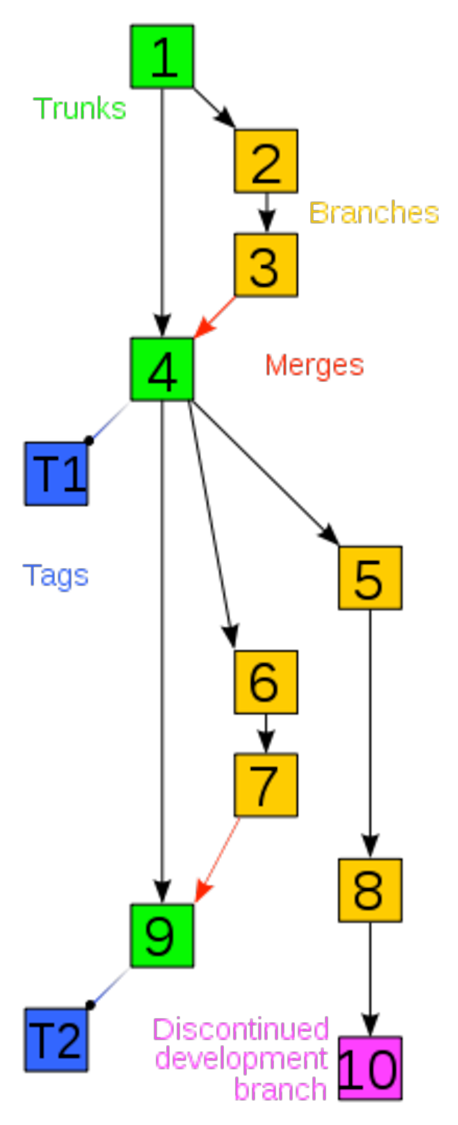
\includegraphics{220px-Revision_controlled_project_visualization-2010-24-02.pdf}}\end{center}
\end{frame}

\begin{frame}
  \frametitle{バージョン管理システムを使うと}
  \begin{center}
    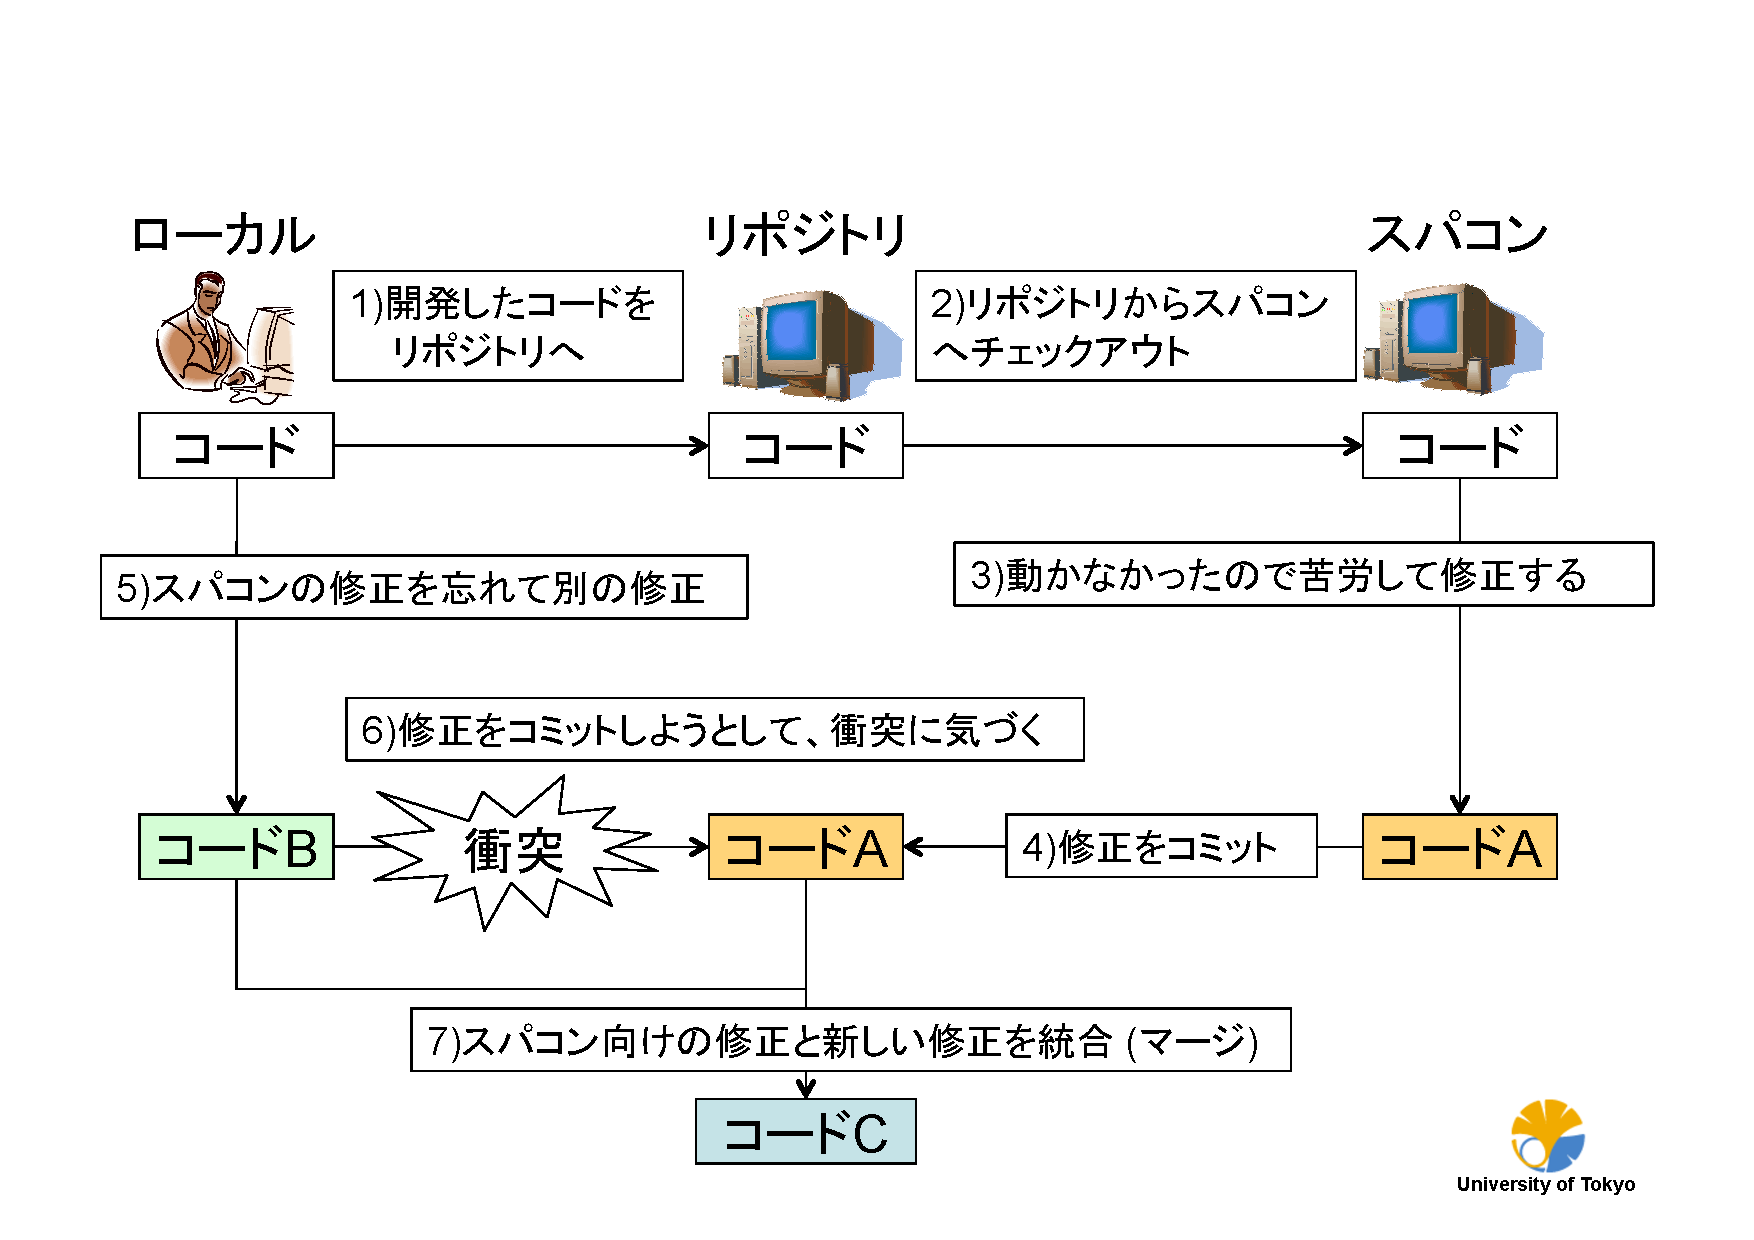
\includegraphics[height=0.78\textheight]{pattern-2.pdf}
  \end{center}
\end{frame}

\begin{frame}[t,fragile]{diff と patch}
  \begin{itemize}
    \setlength{\itemsep}{1em}
  \item {\tt diff}: 2つのテキストファイルの差分を出力するコマンド
    \begin{itemize}
    \item ファイル全体を保存するよりコンパクト
    \item 変更点を確認しやすい
      
      {\tt \$ \underline{diff -u file1.txt file2.txt > file.diff}}
    \end{itemize}
  \item {\tt patch}: {\tt diff}コマンドが生成した差分をファイルに適用するユーティリティー
    \begin{itemize}
    \item もとのファイルと差分から変更後のファイルを生成できる

      {\tt \$ \underline{patch < file.diff}}
    \end{itemize}
  \end{itemize}
\end{frame}

\begin{frame}[t,fragile]
  \frametitle{実習: diff \& patch (1)}
  \begin{itemize}
    %\setlength{\itemsep}{1em}
  \item 単一ファイルの例
\begin{lstlisting}
$ cp /somewhere/diff/prologue.txt prologue.txt
$ cp prologue.txt prologue-orig.txt
$ vi prologue.txt  # prologue.txt を編集

$ diff -u prologue-orig.txt prologue.txt > prologue.diff
$ less prologue.diff
# prologue.diffの中身を見てみる
  
$ cp /somewhere/diff/prologue.txt prologue.txt
$ patch < prologue.diff
$ less prologue.txt  # prologue.txtの中身を確認
\end{lstlisting}
  \end{itemize}
\end{frame}

\begin{frame}[t,fragile]
  \frametitle{実習: diff \& patch (2)}
  \begin{itemize}
    %\setlength{\itemsep}{1em}
  \item ディレクトリ全体を扱う例
\begin{lstlisting}
$ cp -r /somewhere/shake shake
$ cp -r shake shake.orig
# shakeの中のファイルを編集(ファイルの削除や追加も可)

$ diff -urN shake.orig shake > shake.diff
$ less shake.diff   # shake.diffの中身を見てみる

$ rm -rf shake
$ cp -r /somewhere/shake shake
$ patch -p0 < shake.diff
# shakeの中身を確認
\end{lstlisting}
  \item diff と patch で差分の管理は可能になるが, 履歴は別に管理してお
    かなければならない
  \end{itemize}
\end{frame}

\begin{frame}
  \frametitle{主なバージョン管理システム}
  \begin{itemize}
  \item BitKeeper - かつて Linux のカーネルのソース管理に使われていた
  \item CVS (Concurrent Versions System) - ネットワークでの利用を考慮とした初めてのバージョン管理システム. 以前はよく使われていた
  \item Git - 現在 Linux の開発に使われている. 分散型リポジトリ
  \item Mercurial - Git のライバル. 分散型リポジトリ
  \item SCCS (Source Code Control System) - 70年代にベル研で開発された世界初のバージョン管理システム. 現在は使われない
  \item Subversion - CVSの改良版として開発された. 現在最もポピュラー? Mac OS X や多くの Linux には最初からインストールされている
  \end{itemize}
\end{frame}

\begin{frame}
  \frametitle{バージョン管理システムの欠点(面倒な点)}
  \begin{itemize}
  \item 修正前に最新の状態にアップデートしなければならない \\
   ⇒ 慣れると習慣になります
  \item 全ての修正を「コミット」しなければならない \\
    ⇒ 慣れると習慣になります
  \item 衝突(コンフリクト)が発生した時に対処しなければならない \\
    ⇒ 衝突に気づかずに修正してしまうほうが怖いです
  \item サーバのセットアップが面倒くさい \\
    ⇒ まずはホスティングサービス(GitHub, sourceforge, bitbucket)を試してみましょう \\
    ⇒ まわりにいるプロ(?)に相談しましょう \\[.5em]
  \item バージョン管理システムを使うと作業効率が倍以上になる \\
    ⇒ {\color{red} 使わないと人生を半分損する}
  \end{itemize}
\end{frame}

\section{gitの基礎}

\begin{frame}
  \frametitle{gitの基礎}
  \begin{itemize}
  \item 「いつやるの? git入門」\\ \url{http://www.slideshare.net/matsukaz/git-28304397}
    \begin{itemize}
    \item Gitの全体図: \href{http://www.slideshare.net/matsukaz/git-28304397/33}{ページ33--41}      
    \item Gitの内部構造:  \href{http://www.slideshare.net/matsukaz/git-28304397/61}{ページ61--115}
    \end{itemize}
  \end{itemize}
\end{frame}

\begin{frame}[t,fragile]
  \frametitle{実習: gitの基礎(1)}
  \begin{itemize}
  \item ユーザ名などの設定(ログなどに使用される)
\begin{lstlisting}
$ git config --global user.name 'XXXX YYYY'
$ git config --global user.email xxx@yyy.zz
\end{lstlisting}
  \item 作業用ディレクトリとgitリポジトリの作成
\begin{lstlisting}
$ mkdir myproject
$ cd myproject
$ git init
Initialized empty Git repository in /home/xxx/myproject/.git/
$ ls -a
.	..	.git
\end{lstlisting}
  全ての履歴情報は .git に保存される. けっして .git を消さないように!
  \end{itemize}
\end{frame}

\begin{frame}[t,fragile]
  \frametitle{実習: gitの基礎(2)}
  \begin{itemize}
  \item ファイルの作成 \& 管理対象に追加(ステージング)
\begin{lstlisting}
$ vi readme.txt
$ git add readme.txt
$ git status
# On branch master
#
# Initial commit
#
# Changes to be committed:
#   (use "git rm --cached <file>..." to unstage)
#
#	new file:   readme.txt
#
\end{lstlisting}
  \end{itemize}
\end{frame}

\begin{frame}[t,fragile]
  \frametitle{実習: gitの基礎(3)}
  \begin{itemize}
  \item リポジトリに登録(コミット)
\begin{lstlisting}
$ git commit -m 'Initial commit'
[master (root-commit) 5714b10] Initial commit
 0 files changed
 create mode 100644 readme.txt
$ git status
# On branch master
nothing to commit (working directory clean)
\end{lstlisting}
  メッセージ中の``5714b10''がコミットID(の最初の何文字か)
  \end{itemize}
\end{frame}

\begin{frame}[t,fragile]
  \frametitle{実習: gitの基礎(4)}
  \begin{itemize}
  \item ファイルを編集
\begin{lstlisting}
$ vi readme.txt
\end{lstlisting}
  \item 差分を見てみる
\begin{lstlisting}
$ git diff
diff --git a/readme.txt b/readme.txt
index eaf543d..c337c4e 100644
--- a/readme.txt
+++ b/readme.txt
@@ -1 +1,2 @@
 Example of readme file.
+Added a new line.
\end{lstlisting}
  \end{itemize}
\end{frame}

\begin{frame}[t,fragile]
  \frametitle{実習: gitの基礎(5)}
  \begin{itemize}
  \item ステータスを確認
\begin{lstlisting}
$ git status
# On branch master
# Changes not staged for commit:
#   (use "git add <file>..." to update what will be committed)
#   (use "git checkout -- <file>..." to discard changes in working directory)
#
#	modified:   readme.txt
#
no changes added to commit (use "git add" and/or "git commit -a")
\end{lstlisting}
  \end{itemize}
\end{frame}

\begin{frame}[t,fragile]
  \frametitle{実習: gitの基礎(6)}
  \begin{itemize}
  \item ステージング, コミット
\begin{lstlisting}
$ git add readme.txt
$ git commit -m 'Added one line.'
[master c498a65] Added one line.
 1 file changed, 1 insertion(+)
\end{lstlisting}
  \item ログの確認
\begin{lstlisting}
$ git log
commit c498a65ae0a267c206ab1e89fbdb6cfc31d56f2f
Author: Synge Todo <wistaria@issp.u-tokyo.ac.jp>
Date:   Wed Aug 11 22:37:03 2013 +0900

    Added one line.
...
\end{lstlisting}
  \end{itemize}
\end{frame}

\begin{frame}[t,fragile]
  \frametitle{実習: gitの基礎(7)}
  \begin{itemize}
  \item 新しいファイルの作成, ステージング, コミット
\begin{lstlisting}
$ vi hello.txt
$ git add hello.txt
$ git commit -m 'Created hello.txt'
\end{lstlisting}
  \item サブディレクトリの下にファイルを作成
\begin{lstlisting}
$ mkdir src
$ vi src/myprog.f
$ git add src/myprog.f
$ git commit -m 'Initial version of myprog.f'
\end{lstlisting}
  \item ファイルの削除, 移動, コミット間の差分
  \end{itemize}
\end{frame}

\section{ブランチとマージ}

\begin{frame}
  \frametitle{ブランチとマージ}
  \begin{itemize}
    \setlength{\itemsep}{1em}
  \item 「いつやるの? git入門」\\ {\footnotesize \url{http://www.slideshare.net/matsukaz/git-28304397}}
    \begin{itemize}
    \item ブランチとは: \href{http://www.slideshare.net/matsukaz/git-28304397/119}{ページ119--136}      
    \item ブランチを操作してみよう: \href{http://www.slideshare.net/matsukaz/git-28304397/144}{ページ144--157}
    \end{itemize}
  \item ブランチを統合するには「マージ(merge)」と「リベース(rebase)」の2つの方法がある
    \begin{itemize}
    \item mergeのみで十分. また, rebaseは使い方を誤ると危険なので本実習では触れない \\
    \item 参考:「こわくないGit」\\
      \url{http://www.slideshare.net/kotas/git-15276118}
    \end{itemize}
  \end{itemize}
\end{frame}

\begin{frame}[t,fragile]
  \frametitle{実習: ブランチとマージ(1)}
  \begin{itemize}
  \item develop ブランチの作成
\begin{lstlisting}
$ git branch develop
$ git checkout develop
Switched to branch 'develop'
$ git branch
* develop
  master
\end{lstlisting}
  \item develop ブランチに doc.txt を作成
\begin{lstlisting}
$ vi doc.txt
$ git add doc.txt
$ git commit -m 'Created documentation'
[develop 9b5f323] Created documentation
 1 file changed, 1 insertion(+)
 create mode 100644 doc.txt
\end{lstlisting}
  \end{itemize}
\end{frame}

\begin{frame}[t,fragile]
  \frametitle{実習: ブランチとマージ(2)}
  \begin{itemize}
  \item masterブランチに戻ってみる
\begin{lstlisting}
$ git checkout master
$ ls
hello.txt	readme.txt	src
\end{lstlisting}
doc.txt がなくなっていることに注意 \\[.5em]
  \item もう一度, developブランチに切り替え
\begin{lstlisting}
$ git checkout develop
$ ls
doc.txt		hello.txt	readme.txt	src
\end{lstlisting}
  \end{itemize}
\end{frame}

\begin{frame}[t,fragile]
  \frametitle{実習: ブランチとマージ(3)}
  \begin{itemize}
  \item masterブランチでファイルを編集, コミット
\begin{lstlisting}
$ git checkout master
$ vi hello.txt
$ git add hello.txt
$ git commit -m 'Modified hello.txt'
\end{lstlisting}
この時点で master と develop が枝分かれ! \\[.5em]
  \item developブランチをmasterブランチにマージ
\begin{lstlisting}
$ git merge develop
Merge made by the 'recursive' strategy.
 doc.txt |    1 +
 1 file changed, 1 insertion(+)
 create mode 100644 doc.txt
\end{lstlisting}
  \end{itemize}
\end{frame}

\begin{frame}[t,fragile]
  \frametitle{実習: ブランチとマージ(4)}
  \begin{itemize}
  \item コミットグラフ(の一部)を表示
\begin{lstlisting}
$ git log --graph
...
\end{lstlisting}
GitHub (後述)を使っている場合には, ブラウザでコミットグラフを見ることができる
  \end{itemize}
\end{frame}

\begin{frame}[t,fragile]
  \frametitle{実習: ブランチとマージ(5)}
  \begin{itemize}
  \item 今度はコンフリクトが起こるような修正を行ってみる
\begin{lstlisting}
$ git checkout develop
$ vi hello.txt  # 先程と同じ場所を違う文字列に修正
$ git add hello.txt
$ git commit -m 'Modified hello.txt differently'
\end{lstlisting}
  \item マージしようとすると失敗する!
\begin{lstlisting}
$ git checkout master
Switched to branch 'master'
$ git merge develop
Auto-merging hello.txt
CONFLICT (content): Merge conflict in hello.txt
Automatic merge failed; fix conflicts and then commit the result.
\end{lstlisting}
  \end{itemize}
\end{frame}

\begin{frame}[t,fragile]
  \frametitle{実習: ブランチとマージ(6)}
  \begin{itemize}
  \item hello.txtの中を見るとコンフリクトした箇所がわかる
\begin{lstlisting}
$ cat hello.txt
<<<<<<< HEAD
hello, CMSI
=======
hello, MateriApps
>>>>>>> develop
\end{lstlisting}
'\verb+<<<<<<<+'と'\verb+>>>>>>>+'の間の領域がコンフリクト \\[.0em]
  \item ファイルを編集してコンフリクトを解消, コミット
\begin{lstlisting}
$ vi hello.txt
$ cat hello.txt
hello, MateriApps
$ git add hello.txt
$ git commit -m 'Merge branch develop'
\end{lstlisting}
  \end{itemize}
\end{frame}

\section{リモートリポジトリとの連携}

\begin{frame}
  \frametitle{リモートリポジトリとの連携}
  \begin{itemize}
  \item 「いつやるの? git入門」ページ161--208 \\
    \url{http://www.slideshare.net/matsukaz/git-28304397}
  \end{itemize}
\end{frame}

\begin{frame}[t,fragile]
  \frametitle{実習: リモートリポジトリとの連携(1)}
  \begin{itemize}
  \item 実習で用いるGitHub上のリモートリポジトリ git@github.com:cmsi/vcs-hands-on.git
  \item ブラウザでのアクセス \url{https://github.com/cmsi/vcs-hands-on}
  %\item (時間があれば)「Git道場 技 本日の課題,  テクニックの解説」 \\
    % \url{https://speakerdeck.com/ogawa/git} に従って演習
  \item リモートリポジトリをローカルに複製
\begin{lstlisting}
$ git clone git@github.com:cmsi/vcs-hands-on.git
Cloning into 'vcs-practice'...
remote: Counting objects: 4, done.
remote: Compressing objects: 100% (4/4), done.
remote: Total 4 (delta 0), reused 4 (delta 0)
Receiving objects: 100% (4/4), done.
\end{lstlisting}
  \end{itemize}
\end{frame}

\begin{frame}[t,fragile]
  \frametitle{実習: リモートリポジトリとの連携(2)}
  \begin{itemize}
  \item 課題1: 自分のページの作成
    \begin{itemize}
      \item todo.html を自分の名前にコピーして編集
\begin{lstlisting}
$ cd vcs-hands-on
$ cp todo.html igarashi.html
$ vi igarashi.html
\end{lstlisting}
      \item index.html を編集し, 自分のページヘのリンクを作成
      \item ローカルリポジトリにコミット
      \item リモートリポジトリにプッシュ
\begin{lstlisting}
$ git push origin master
\end{lstlisting}
    \end{itemize}
  \end{itemize}
\end{frame}

\begin{frame}[t,fragile]
  \frametitle{実習: リモートリポジトリとの連携(3)}
  \begin{itemize}
  \item 課題2: 他の人のページから自分のページへのリンクの作成
    \begin{itemize}
      \item リモートブランチ(origin/master)を最新版に更新し, masterにマージ
\begin{lstlisting}
$ git fetch
$ git merge origin/master
\end{lstlisting}
      \item 誰かのページを編集. 自分のページヘのリンクを作成
      \item ローカルリポジトリにコミット
      \item リモートリポジトリにプッシュ
    \end{itemize}
  \end{itemize}
\end{frame}

\begin{frame}[t,fragile]
  \frametitle{実習: リモートリポジトリとの連携(4)}
  \begin{itemize}
  \item プッシュが失敗した場合
    \begin{itemize}
      \item 誰かがすでにプッシュしている
      \item まずリモートリポジトリの内容をマージしてから再度プッシュ
\begin{lstlisting}
$ git fetch
$ git merge origin/master
$ git push origin master
\end{lstlisting}
    \end{itemize}
  \item マージの際にコンフリクトした場合
    \begin{itemize}
      \item ファイルを修正しコミットした後, プッシュ
    \end{itemize}
  \item コミットグラフの確認
\begin{lstlisting}
$ git log --graph
\end{lstlisting}
    あるいはブラウザで\url{https://github.com/cmsitest/vcs-practice/network}にアクセス
  \end{itemize}
\end{frame}

\begin{frame}
  \frametitle{gitワークフローのまとめ}
  \begin{center}
    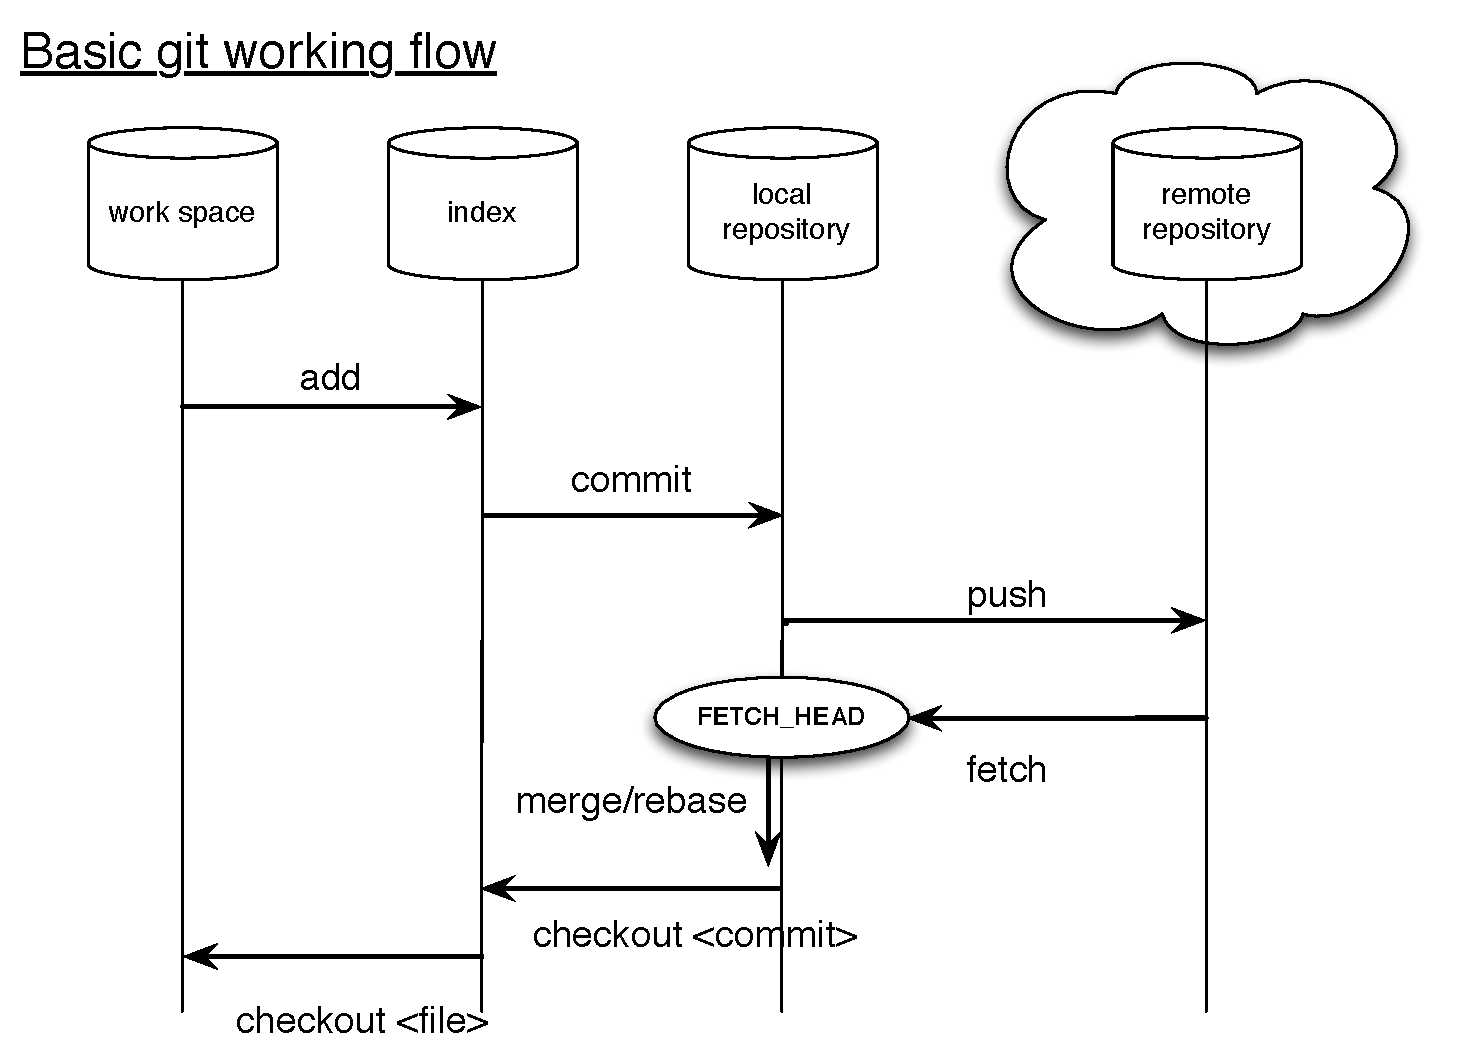
\includegraphics[height=.8\textheight]{../workflow/git-diagram.pdf}
  \end{center}
\end{frame}

\begin{frame}
  \frametitle{バージョン管理システムを使う上での注意点}
  \begin{itemize}
    \setlength{\itemsep}{1em}
  \item gitが管理している領域からファイルを持ちだして編集してはいけない
  \item 大きなバイナリファイル(pdf, exe, doc, tar.gz, zipなど)をgitで管理しない
  \end{itemize}
\end{frame}

\section{GitHubを用いたオープンソース・ソフトウェアの開発・公開}

\begin{frame}
  \frametitle{「公開ソフト」に必要なもの}
  \begin{itemize}
  \item マニュアル
  \item チュートリアル
  \item ライセンス
  \item ビルドシステム and/or インストーラー
    \begin{itemize}
    \item ソースコード配布 \\
      Linuxで一般的. ソースと一緒にビルド環境(Makefile, CMake, configure スクリプト)を配布
    \item バイナリ配布 \\
      Windowsで一般的. バイナリインストーラー形式で配布
    \end{itemize}
  \item ユーザフレンドリな操作環境(GUIなど)
  \item ユーザサポート体制
  \end{itemize}
\end{frame}

\begin{frame}
  \frametitle{ビルドシステム: CMake}
  \begin{itemize}
    \setlength{\itemsep}{1em}
  \item Makefileを生成するためのユーティリティー (configureスクリプトに対応)
    \begin{itemize}
    \item Windows の Visual C++ 用ソリューションファイル, Mac OS X の Xcode 用プロジェクトファイルの生成も可能
    \end{itemize}
  \item 設定は CMakeLists.txt に記述する
  \item テスト(CTest)やバイナリインストーラ作成(CPack)の機能もある
  \item ファイルの依存関係の自動検出
  \item 必要なライブラリ(MPI, LAPACK等)の検索機能
  \end{itemize}
\end{frame}

\begin{frame}
  \frametitle{オープンソース・ソフトウェア開発の流れ (例)}
  \begin{itemize}
    %\setlength{\itemsep}{1em}
  \item GitHub にリポジトリを作成
  \item 開発
    \begin{itemize}
    \item ソースコード
    \item ビルドシステム
    \item ドキュメント類
    \item テスト
    \end{itemize}
  \item バージョン番号を割り当て
  \item 公開
    \begin{itemize}
    \item 配布物の作成 (tar.gz, インストーラー)
    \item 配布物のアップロード
    \item アナウンス
    \end{itemize}
  \item 次期バージョンの開発へ
  \end{itemize}
\end{frame}

\begin{frame}[t,fragile]
  \frametitle{実習: GitHubを用いたオープンソース・ソフトウェアの開発・公開(1)}
  \begin{itemize}
  \item GitHubで新しいリポジトリを作成
    \begin{itemize}
      \item \url{https://github.com}にログインし, 右上の``Create a new repo''をクリック
      \item リポジトリのURLは, ページ右下の``SSH clone URL''に表示されている
    \end{itemize}
  \item GitHub上のリポジトリをローカルに複製
\begin{lstlisting}
$ git clone git@github.com:foo/myproject.git  # 例
\end{lstlisting}
  \item ソースコードを作成
\begin{lstlisting}
$ cd myproject
$ vi hello.f90  # Fortranの場合
$ vi hello.cpp  # C++の場合
\end{lstlisting}
  ソースコードの例: \url{https://github.com/cmsi/vcs-tutorial/tree/develop/opensource}
  \end{itemize}
\end{frame}

\begin{frame}[t,fragile]
  \frametitle{実習: GitHubを用いたオープンソース・ソフトウェアの開発・公開(2)}
  \begin{itemize}
  \item ソースコードをローカルリポジトリにコミット
  \item リモートリポジトリにプッシュ
  \item CMakeLists.txtの作成 (例: Fortranの場合)
\begin{lstlisting}
cmake_minimum_required(VERSION 2.8 FATAL_ERROR)
project(hello NONE)      # プロジェクト名

enable_language(Fortran) # 使用する言語

# 作成するバイナリ名とそれに必要なソースファイル名
add_executable(hello hello.f90)
\end{lstlisting}
  \end{itemize}
\end{frame}

\begin{frame}[t,fragile]
  \frametitle{実習: GitHubを用いたオープンソース・ソフトウェアの開発・公開(3)}
  \begin{itemize}
  \item CMakeLists.txtの作成 (例: C++の場合)
\begin{lstlisting}
cmake_minimum_required(VERSION 2.8 FATAL_ERROR)
project(hello NONE)  # プロジェクト名

enable_language(C++) # 使用する言語

# 作成するバイナリ名とそれに必要なソースファイル名
add_executable(hello hello.cpp)
\end{lstlisting}
  ソースファイルが複数ある場合は, それらを列挙すれば良い \\[0.5em]
  \item CMakeLists.txtをローカルリポジトリにコミット, リモートリポジトリにプッシュ
  \end{itemize}
\end{frame}

\begin{frame}[t,fragile]
  \frametitle{実習: GitHubを用いたオープンソース・ソフトウェアの開発・公開(4)}
  \begin{itemize}
  \item ソースコード, CMakeLists.txtのテスト
\begin{lstlisting}
$ mkdir myproject-build  # gitで管理しているディレクトリの外でテスト
$ cd myproject-build
$ cmake $HOME/myproject  # gitで管理しているディレクトリを指定
$ make                   # helloがビルドされる
$ ./hello
hello, world
\end{lstlisting}
  \item さらにドキュメント, ライセンスファイルなどを追加
  \end{itemize}
\end{frame}

\begin{frame}[t,fragile]
  \frametitle{実習: GitHubを用いたオープンソース・ソフトウェアの開発・公開(5)}
  \begin{itemize}
  \item リリース作業
    \begin{itemize}
    \item 必要なファイル, 修正を全てコミット
    \item タグをつけ, リモートにプッシュ
\begin{lstlisting}
$ git tag -a 1.0
$ git tag  # タグの確認
$ git push origin 1.0
\end{lstlisting}
    \end{itemize}
  \item GitHubでは、タグをつけると「リリース」として一覧に現れる
    \begin{itemize}
    \item 「releases」タブをクリックするとリリース一覧が表示される
    \item ソースコード(tar.gz形式、zip形式)へのリンクが自動的に作成される
    \end{itemize}
  \end{itemize}
\end{frame}

\begin{frame}[t,fragile]
  \frametitle{実習: GitHubを用いたオープンソース・ソフトウェアの開発・公開(6)}
  \begin{itemize}
    \setlength{\itemsep}{1em}
  \item 配布物にソースコード以外(バイナリ、マニュアルPDFなど)を含めたい場合
    \begin{itemize}
    \item いったんアーカイブを作成
\begin{lstlisting}
$ git archive --format tar --prefix=myproject-1.0/ 1.0 | gzip > myproject-1.0.tar.gz
$ git archive --format zip --prefix=myproject-1.0/ 1.0 > myproject-1.0.zip
\end{lstlisting}
    \item 必要なファイルを追加したのち、「リリース」の編集ページでファイルを追加する
    \end{itemize}
  \item リリースノートの更新, アナウンス
    \begin{itemize}
    \item MateriApps, github.io, twitter などを活用
    \end{itemize}
  \end{itemize}
\end{frame}

\section{その他}

\begin{frame}
  \frametitle{その他の話題}
  \begin{itemize}
    \setlength{\itemsep}{1em}
  \item A successful Git branching model (ブランチの上手な使い方) \url{http://keijinsonyaban.blogspot.jp/2010/10/successful-git-branching-model.html}
  \item Gitをボトムアップから理解する (gitの中で何が起こっているのかを知りたい人向け) 
    \url{http://keijinsonyaban.blogspot.jp/2011/05/git.html}
  \end{itemize}
\end{frame}

\end{document}
